\documentclass[conference,a4paper]{IEEEtran}
\IEEEoverridecommandlockouts

% Standard IEEE conference packages
\usepackage[T1]{fontenc}
\usepackage{cite}
\usepackage{amsmath,amssymb,amsfonts}
\usepackage{algorithmic}
\usepackage{graphicx}
\usepackage{textcomp}
\usepackage{xcolor}
\usepackage{booktabs}
\usepackage{tabularx}
\usepackage{multirow}
\usepackage{url}
\usepackage{microtype}
\usepackage{enumitem}
\setlist{nosep, leftmargin=*, topsep=1.0pt, partopsep=0pt, parsep=0pt, itemsep=0.5pt}

% Ensure figures subfolder is searchable
\graphicspath{{figures/}{./}}

% Compact float and equation spacing for strict 8-page conference limit on A4 paper
\setlength{\textfloatsep}{2.5pt plus 0.5pt minus 0.5pt}
\setlength{\floatsep}{2.0pt plus 0.5pt minus 0.5pt}
\setlength{\intextsep}{2.0pt plus 0.5pt minus 0.5pt}
\setlength{\dbltextfloatsep}{2.5pt plus 0.5pt minus 0.5pt}
\setlength{\dblfloatsep}{2.0pt plus 0.5pt minus 0.5pt}
\setlength{\abovecaptionskip}{1.5pt}
\setlength{\belowcaptionskip}{1.5pt}
\setlength{\abovedisplayskip}{1.5pt plus 0.5pt minus 0.5pt}
\setlength{\belowdisplayskip}{1.5pt plus 0.5pt minus 0.5pt}
\renewcommand{\topfraction}{0.95}
\renewcommand{\dbltopfraction}{0.95}
\renewcommand{\bottomfraction}{0.95}
\renewcommand{\textfraction}{0.05}
\renewcommand{\baselinestretch}{0.960}

\begin{document}

\title{Spatial Evidence Traceability in Multimodal Document RAG: A Systematic Review of Region-Level Provenance, Cross-Page Retrieval, and Claim Attribution}

\author{
\IEEEauthorblockN{Shambhuraje Jadhav\IEEEauthorrefmark{1}, Amol Kanherkar\IEEEauthorrefmark{1}, Vaishnavi Ghode\IEEEauthorrefmark{1}, Aarti Kalyane\IEEEauthorrefmark{1}, and Hema Jadhav\IEEEauthorrefmark{2}}
\IEEEauthorblockA{Department of Artificial Intelligence and Data Science\\
Vidya Pratishthan's Kamalnayan Bajaj Institute of Engineering and Technology (VPKBIET), Baramati\\
Savitribai Phule Pune University (SPPU), Pune, Maharashtra 413133, India\\
Email: \IEEEauthorrefmark{1}\{shambhuraje.jadhav.aids.2023, amol.kanherkar.aids.2023, vaishnavi.ghode.aids.2023, aarti.kalyane.aids.2023\}@vpkbiet.org, \IEEEauthorrefmark{2}hema.jadhav@vpkbiet.org}
}

\maketitle

\begin{abstract}
\mdseries
Complex enterprise documents---such as financial filings, clinical study protocols, engineering blueprints, and legal contracts---encode critical domain knowledge across multi-page visual layouts, 2D tabular grids, and infographics. While Retrieval-Augmented Generation (RAG) mitigates large language model hallucinations, conventional architectures rely on 1D text chunking and dense vector similarity. This design shears tabular records, discards visual coordinates, and obscures the provenance chain linking generated claims back to original document regions. To our knowledge, this review provides one of the first structured analyses of spatial provenance, cross-page evidence retrieval, and claim-level attribution within multimodal document RAG. Guided by the PRISMA 2020 systematic review methodology, this paper investigates spatial evidence traceability across multimodal document intelligence. From an initial automated harvest of 540 candidate records across four major scientific indexing registries (IEEE Xplore, ACM DL, ACL Anthology, Scopus) executed on November 14, 2026, 532 deduplicated unique records underwent standardized title/abstract double-screening ($503/532 = 94.55\%$ raw agreement, Cohen's $\kappa = 0.8109$), advancing 81 database reports to full-text eligibility appraisal alongside 5 supplementary citation-snowballing sources (86 total assessed, $82/86 = 95.35\%$ raw agreement, $\kappa = 0.9044$). Excluding 36 records yielded exactly 50 synthesized research sources (45 database archival studies $+ 5$ supplementary citation-snowballing sources), stratified into 23 core primary empirical systems and 27 supporting literature sources (benchmarks, surveys, foundational baselines, guidelines). We formulate a five-stage Evidence Lifecycle Framework ($\mathcal{S}_1$--$\mathcal{S}_5$) to systematically map where information loss occurs and how it can be mitigated. We formalize operational tabular integrity metrics (Cell Integrity Ratio and Row Continuity Ratios), formulate multi-hop graph exploration via deterministic matrix computation of finite-horizon discounted stochastic propagation, and audit nine benchmarks relevant to document retrieval, multimodal grounding, multi-hop reasoning, and claim attribution across four explicit dimensions. Finally, we synthesize architectural design principles into Layout-Aware Multimodal GraphRAG (LAM-GraphRAG), outlining an open research agenda for verifiable, provenance-grounded multimodal document understanding.
\end{abstract}

\begin{IEEEkeywords}
Multimodal Document Intelligence, Evidence Traceability, Spatial Provenance, Retrieval-Augmented Generation (RAG), GraphRAG, Multi-Hop Reasoning, Claim Attribution.
\end{IEEEkeywords}

%========================================================================================
% SECTION I: INTRODUCTION & PROBLEM STATEMENT
%========================================================================================
\section{Introduction and Problem Statement}
Large Language Models (LLMs) demonstrate remarkable generative proficiency across natural language processing benchmarks \cite{brown2020}. However, when deployed in mission-critical enterprise environments, LLMs exhibit a persistent failure mode: hallucinations \cite{ji2023}. To mitigate ungrounded generations, Retrieval-Augmented Generation (RAG) has emerged as the operational standard \cite{lewis2020, guu2020}. Conventional RAG relies on serialized 1D text chunking (typically 256--512 tokens) and dense vector similarity. When applied to visually rich enterprise documents (PDFs, spreadsheets, contracts), this induces four systemic failure modes:
\begin{enumerate}
    \item[(a)] \textbf{Tabular Relational Fracture:} Fixed-window chunking slices across tabular rows blindly, severing cell values from hierarchical headers;
    \item[(b)] \textbf{Spatial Geometry Loss:} Discarding 2D coordinate bounding boxes ($[x_0, y_0, x_1, y_1, p]$) destroys spatial proximity and multi-column reading orders;
    \item[(c)] \textbf{Multi-Hop Cross-Page Blindness:} Independent top-$k$ retrieval often fails to reconstruct distributed reasoning chains that span multiple pages \cite{yang2018hotpotqa, trivedi2023}; and
    \item[(d)] \textbf{Absence of Coordinate Provenance:} Generated claims cite coarse document passages rather than auditable, bounding-box physical regions \cite{tripathi2026, yang2025adaptiveguard}.
\end{enumerate}

To our knowledge, this review provides one of the first structured analyses of spatial evidence traceability across multimodal document intelligence. Our core contributions are:
\begin{itemize}
    \item \textbf{PRISMA 2020 Systematic Protocol:} A structured systematic review synthesizing 50 research sources (45 database archival publications + 5 supplementary citation-snowballing sources) from 540 initial records, adhering to dual-pathway PRISMA 2020 guidelines \cite{page2021prisma}.
    \item \textbf{Evidence Lifecycle Framework ($\mathcal{S}_1$--$\mathcal{S}_5$):} A five-stage formalization mapping evidence loss from visual layout perception to claim attribution.
    \item \textbf{Relational Tabular Preservation Metrics:} Novel operational formulations---Cell Integrity Ratio ($\text{CIR}_{\text{logical}}$, $\text{CIR}_{\text{data}}$) and Row Continuity Ratios (H-RCR, C-RCR)---quantifying structural preservation under chunking.
    \item \textbf{Bounded Topological Exploration:} A deterministic finite-horizon matrix propagation formulation bounding multi-hop exploration strictly to $O(K \cdot |\mathcal{E}|)$ complexity.
    \item \textbf{Decoupled Evaluation Taxonomy \& LAM-GraphRAG Architecture:} Auditing nine representative benchmarks across four decoupled dimensions and proposing Layout-Aware Multimodal GraphRAG (LAM-GraphRAG) with auditable coordinate provenance.
\end{itemize}

%========================================================================================
% SECTION II: BACKGROUND & CONCEPTUAL FOUNDATIONS
%========================================================================================
\section{Background and Conceptual Foundations}

\subsection{1D RAG vs. Spatial Evidence Provenance}
Standard RAG retrieves top-$k$ text chunks using dense vector cosine similarity $\cos(\mathbf{e}_q, \mathbf{e}_{c_i})$ to prompt LLMs \cite{brown2020, devlin2019, lewis2020, guu2020}. While effective for linear prose, this paradigm assumes text invariance to layout geometry. Visually rich enterprise documents encode critical relationships across 2D grids, multi-column flows, and visual hierarchies \cite{radford2021, liu2023llava}. Serializing pages into 1D token streams shears relational dependencies and induces ``Lost in the Middle'' retrieval blindspots \cite{liu2024lost}.

\subsection{The Five-Stage Evidence Lifecycle Framework}
To map where information fractures, we establish a five-stage Evidence Lifecycle Framework ($\mathcal{S}_1$--$\mathcal{S}_5$): (1)~\textbf{Visual \& Layout Perception ($\mathcal{S}_1$):} multi-format ingestion and bounding-box segmentation; (2)~\textbf{Hierarchical Chunking \& Coordinate Grounding ($\mathcal{S}_2$):} cell-to-header binding and immutable spatial coordinate registration; (3)~\textbf{Cross-Page \& Multimodal Graph Indexing ($\mathcal{S}_3$):} structuring text, tables, and figures into typed graph topologies; (4)~\textbf{Uncertainty-Aware Multi-Hop Retrieval ($\mathcal{S}_4$):} bounded graph traversal and epistemic uncertainty arbitration; and (5)~\textbf{Claim Attribution Layer ($\mathcal{S}_5$):} auditing generated statements against verified coordinate regions.

\subsection{Comparison with Existing Literature Surveys}
Several recent surveys review RAG components; however, none provides formal integrated coverage across all five spatial lifecycle stages. Table~\ref{tab:survey_comparison} summarizes related surveys evaluated via independent double-coding ($22/25 = 88.00\%$ raw agreement, $\kappa = 0.8005$). While Gao et al.~\cite{gao2026} survey vision-language models for page-level visual retrieval, they evaluate documents at whole-page granularity and do not address sub-page coordinate bounding boxes, 2D tabular cell integrity, or graph multi-hop evidence chains. Peng et al.~\cite{peng2025} and Li et al.~\cite{li2025} evaluate textual GraphRAG and long-context LLMs, discarding 2D layout geometry; Zhang~\cite{zhang2025} addresses single-page MLLM parsing without cross-page graph traversal; and Ni et al.~\cite{ni2026trustworthy} review general RAG trustworthiness without spatial bounding boxes. In contrast, our review focuses specifically on fine-grained region-level provenance, cross-page graph reasoning, and spatial claim attribution across the full five-stage evidence lifecycle.

\begin{table}[htbp]
\caption{Coverage of Evidence Lifecycle Stages Across Related Surveys.}
\centering
\scriptsize
\setlength{\tabcolsep}{1.2pt}
\begin{tabularx}{\columnwidth}{@{}p{2.3cm}ccccc>{\raggedright\arraybackslash}X@{}}
\toprule
\textbf{Survey Reference} & \textbf{$\mathcal{S}_1$} & \textbf{$\mathcal{S}_2$} & \textbf{$\mathcal{S}_3$} & \textbf{$\mathcal{S}_4$} & \textbf{$\mathcal{S}_5$} & \textbf{Primary Focus \& Technical Gap} \\
\midrule
Gao et al. (2026) \cite{gao2026} & $\circ$ & $\bullet$ & $\times$ & $\bullet$ & $\circ$ & Page-level MLLM; lacks spatial bbox provenance. \\
Peng et al. (2026) \cite{peng2025} & $\times$ & $\times$ & $\times$ & $\bullet$ & $\circ$ & Text GraphRAG; ignores 2D layout geometry. \\
Zhang (2025) \cite{zhang2025} & $\circ$ & $\bullet$ & $\times$ & $\times$ & $\times$ & Single-page parsing; lacks multi-page graph reasoning. \\
Li et al. (2026) \cite{li2025} & $\times$ & $\times$ & $\times$ & $\circ$ & $\times$ & Long-text RAG; omits tabular and visual structures. \\
Ni et al. (2026) \cite{ni2026trustworthy} & $\times$ & $\times$ & $\times$ & $\circ$ & $\bullet$ & Textual trustworthiness; lacks spatial bbox audit. \\
\textbf{This Review (2026)}$^\ddagger$ & $\bullet$ & $\bullet$ & $\bullet$ & $\bullet$ & $\bullet$ & \textbf{Unifies 2D parsing, GraphRAG, \& attribution.} \\
\bottomrule
\end{tabularx}
\vspace{1.5pt}
\begin{minipage}{\columnwidth}
{\scriptsize\raggedright \textbf{Notes:} $\bullet$ = Primary focus; $\circ$ = Partial/secondary coverage; $\times$ = Omitted/out of scope. $^\ddagger$Double-coding agreement: $22/25 = 88.00\%$, Cohen's $\kappa = 0.8005$.\par}
\end{minipage}
\label{tab:survey_comparison}
\end{table}

%========================================================================================
% SECTION III: REVIEW METHODOLOGY (PRISMA 2020 PROTOCOL)
%========================================================================================
\section{Review Methodology (PRISMA 2020 Protocol)}

\subsection{PRISMA Protocol Adherence and Research Questions}
We conducted a structured systematic review following PRISMA 2020 standards \cite{page2021prisma}. Our protocol addresses five research questions:
\begin{itemize}
    \item \textbf{RQ1 (Perception \& Extraction):} How effectively do current document parsers preserve 2D layout coordinates and relational table integrity?
    \item \textbf{RQ2 (Indexing \& Topology):} How do document graph indices balance multi-hop expressive power against index construction overhead?
    \item \textbf{RQ3 (Multi-Hop Retrieval):} How do deterministic matrix walks compare with iterative prompt exploration in accuracy and complexity?
    \item \textbf{RQ4 (Evaluation Dimensions):} To what extent do existing benchmarks decouple spatial coordinate grounding from text citation recall?
    \item \textbf{RQ5 (Architecture \& Provenance):} What modular architecture unifies layout perception, graph propagation, and coordinate claim verification?
\end{itemize}

\subsection{Search Strategy and Dual-Pathway Screening Workflow}
Automated searches were executed on November 14, 2026 across four primary scientific indexing registries: IEEE Xplore ($n=160$), ACM Digital Library ($n=140$), ACL Anthology ($n=130$), and Scopus ($n=110$). Following PRISMA 2020 guidelines \cite{page2021prisma}, queries covered publications from January 2017 to November 2026, restricted to English-language peer-reviewed conference proceedings and journal articles. Table~\ref{tab:search_streams} details the four facet concepts; exact database-specific Boolean queries, field tags, and complete execution logs are openly archived in our open supplementary search audit log repository (\url{https://doi.org/10.5281/zenodo.24434432}). The automated harvest yielded 540 candidate records. Deduplication removed 8 duplicate entries, leaving 532 unique records for independent title/abstract double-screening by Reviewer 1 (S.J.) and Reviewer 2 (V.G.), with Reviewer 3 (A.K.) serving as designated consensus adjudicator for the 29 split evaluations.

\begin{table}[htbp]
\caption{Systematic Review Search Streams and Facet Concepts.}
\centering
\scriptsize
\setlength{\tabcolsep}{3.0pt}
\begin{tabularx}{\columnwidth}{llX}
\toprule
\textbf{Stream} & \textbf{Core Facet} & \textbf{Search Concepts and Keywords} \\
\midrule
Stream 1 & Modality & Multimodal document RAG, PDF, document intelligence, table, visual QA. \\
Stream 2 & Extraction & Layout-aware parsing, 2D grids, tables, charts, visual page retrieval. \\
Stream 3 & Topology & GraphRAG, multi-hop retrieval, pseudo-graph, cross-page document reasoning. \\
Stream 4 & Provenance & Spatial coordinates, bounding box grounding, attribution, citation, faithfulness. \\
\bottomrule
\end{tabularx}
\label{tab:search_streams}
\end{table}

Standardized scope criteria excluded 451 records across four operational categories: Scope 1 (Non-Doc NLP and Dialogue, $n = 176$), Scope 2 (Generic Computer Vision and OCR without retrieval indexing, $n = 146$), Scope 3 (Non-Grounded Prompting and Code Generation, $n = 84$), and Scope 4 (Hardware Edge Optimization and Short Trade Notes, $n = 45$). Screeners achieved substantial inter-rater agreement ($503/532 = 94.55\%$, Cohen's $\kappa = 0.8109$).

\begin{figure}[htbp]
\centering
\scriptsize
\begin{tabularx}{\columnwidth}{|X|}
\hline
\multicolumn{1}{|c|}{\textbf{PRISMA 2020 DUAL-PATHWAY FLOW (Evidence Synthesis)}} \\
\hline
\textbf{Pathway A: Primary Automated Database Queries ($N = 540$, Cutoff: Nov 14, 2026)} \\
$\bullet$~IEEE Xplore ($n = 160$) \quad $\bullet$~ACM Digital Library ($n = 140$) \\
$\bullet$~ACL Anthology ($n = 130$) \quad $\bullet$~Scopus Database ($n = 110$) \\
$\longrightarrow$ Duplicate records removed prior to screening: $n = 8$ \\
$\longrightarrow$ Records screened by title and abstract: $n = 532$ \\
$\quad$ [Excluded: $n = 451$ via Scope 1 ($n=176$), Scope 2 ($n=146$), Scope 3 ($n=84$), Scope 4 ($n=45$)] \\
$\quad$ Reviewer concordance: $503/532 = 94.55\%$, Cohen's $\kappa = 0.8109$ \\
$\longrightarrow$ Database full-text reports assessed for eligibility: $n = 81$ \\
$\quad$ [Excluded with reasons ($n = 36$): E1 ($n=9$), E2 ($n=9$), E3 ($n=9$), E4 ($n=9$)] \\
$\longrightarrow$ Database-derived archival publications retained: $\mathbf{n = 45}$ \\
\hline
\textbf{Pathway B: Supplementary Citation Snowballing Identification ($N = 5$)} \\
$\bullet$~Supplementary citation-snowballing sources identified: $n = 5$ \\
$\longrightarrow$ Full-text reports assessed for eligibility: $n = 5$ (Excluded: $n = 0$) \\
$\longrightarrow$ Supplementary citation-snowballing sources retained: $\mathbf{n = 5}$ \\
\hline
\textbf{Final Converged Synthesis Corpus: $N = 45 + 5 = 50$ Studies} \\
$\bullet$~Group A: Core Primary Empirical Systems ($n = 23$, 20 database + 3 supplementary sources) \\
$\bullet$~Group B: Supporting Literature Sources ($n = 27$, 25 database + 2 supplementary sources): \\
$\quad$ Benchmarks ($n = 7$), Surveys ($n = 7$), Baselines ($n = 9$), Safety ($n = 3$), Guideline ($n = 1$) \\
$\quad$ Reviewer appraisal concordance (86 full-text reports): $82/86 = 95.35\%$, Cohen's $\kappa = 0.9044$ \\
\hline
\end{tabularx}
\vspace{2pt}
\caption{PRISMA 2020 Systematic Search, Screening, and Inclusion Protocol (Dual-Pathway Architecture Reconciling Database and Supplementary Sources).}
\label{fig:prisma_flow}
\end{figure}

The remaining 81 database reports advanced to full-text eligibility appraisal alongside 5 supplementary citation-snowballing sources identified via backward and forward citation snowballing (GraphRAG \cite{edge2024}, DocLayout-YOLO \cite{zhao2024doclayout}, MinerU \cite{wang2024mineru}, M3DocVQA \cite{m3docvqa2025}, MMDocRAG \cite{dong2025mmdocrag}). All 86 full-text reports were independently assessed by Reviewer 1 (S.J.) and Reviewer 3 (A.K., domain specialist in graph topologies and spatial document AI). They agreed on 82 of 86 decisions ($82/86 = 95.35\%$; Cohen's $\kappa = 0.9044$), and Reviewer 2 (V.G.) adjudicated the four disagreements. All five supplementary citation-snowballing sources were retained by both reviewers ($5/5$ agreement, $100\%$). Reviewer 1 and Reviewer 2 conducted the initial title/abstract screening ($503/532 = 94.55\%$, $\kappa = 0.8109$) with Reviewer 3 adjudicating splits; for full-text appraisal, Reviewer 3 joined Reviewer 1 for deep architectural evaluation, while Reviewer 2 served as independent adjudicator. Exactly 36 database records were excluded across four pre-registered criteria ($9$ each): E1 (lack of multimodal/layout awareness), E2 (purely conceptual without reproducible evaluations), E3 (proprietary closed-source benchmarks), and E4 (unreviewed commercial trade whitepapers). Deduplicated inclusions converged to exactly 50 synthesized sources (45 database archival studies $+ 5$ supplementary citation-snowballing sources), as depicted in Fig.~\ref{fig:prisma_flow}.

\subsection{Stratified Methodological Quality Appraisal (MQA)}
Synthesized sources were stratified into two complementary cohorts:
\begin{itemize}
    \item \textbf{Group A (Core Primary Empirical Systems, $n=23$):} 20 database archival studies plus 3 supplementary sources (GraphRAG \cite{edge2024}, DocLayout-YOLO \cite{zhao2024doclayout}, MinerU \cite{wang2024mineru}), quantitatively appraised across six empirical quality anchors ($Q_1$--$Q_6$, score range 0--12): architectural reproducibility ($Q_1$), layout coordinate preservation ($Q_2$), graph multi-hop traversal ($Q_3$), claim attribution ($Q_4$), evaluation rigor ($Q_5$), and open availability ($Q_6$). Mean score: $9.87/12$ ($82.25\%$).
    \item \textbf{Group B (Supporting Literature Sources, $n=27$):} 25 database archival studies plus 2 supplementary sources (M3DocVQA \cite{m3docvqa2025}, MMDocRAG \cite{dong2025mmdocrag}), descriptively appraised across cohort-tailored functional dimensions rather than uniform numerical scoring (avoiding category errors across heterogeneous literature types): Standardized Benchmarks ($n=7$; task grounding, coordinate annotation), Literature Surveys ($n=7$; scope and lifecycle stage coverage), Foundational Baselines ($n=9$; algorithmic novelty and citation impact), Agentic Safety Studies ($n=3$; threat modeling and runtime guardrails), and Reporting Guidelines ($n=1$; PRISMA 2020 protocol compliance). The complete 27-source descriptive appraisal matrix is deposited in supplementary material (\texttt{Group\_B\_Source\_Level\_Appraisal\_Matrix.csv}).
\end{itemize}

%========================================================================================
% SECTION IV: SPATIAL EVIDENCE EXTRACTION & TABULAR INTEGRITY
%========================================================================================
\section{Spatial Evidence Extraction and Representation (RQ1)}

\subsection{Tabular Structural Preservation}
Standard character chunkers slice across tabular rows blindly, severing cell values from column headers \cite{chen2024tablerag}. In a hypothetical 512-token chunking example, the defined logical-binding CIR is 59.09\%, illustrating how separating data rows from their hierarchical headers can reduce contextual integrity. To evaluate tabular preservation rigorously, we formalize three author-proposed operational measures: \textbf{Cell Integrity Ratio (CIR)}, \textbf{Horizontal Row Continuity (H-RCR)}, and \textbf{Contextual Row Continuity (C-RCR)}:
\begin{equation}
\text{CIR}_{\text{logical}} = \frac{N_{\text{intact\_units}}}{N_{\text{total\_units}}}, \quad \text{CIR}_{\text{data}} = \frac{N_{\text{contextual\_data\_cells}}}{N_{\text{total\_data\_cells}}}
\label{eq:cir}
\end{equation}
\begin{equation}
\text{H-RCR} = \frac{N_{\text{horizontally\_intact\_rows}}}{N_{\text{total\_rows}}}
\label{eq:hrcr}
\end{equation}
\begin{equation}
\text{C-RCR} = \frac{N_{\text{rows\_with\_valid\_header\_context}}}{N_{\text{total\_rows}}}
\label{eq:crcr}
\end{equation}
where CIR measures the proportion of logical cell-binding units whose text and header associations remain unsevered. In our formulation: (i)~merged headers are projected into constituent column attribute slots; (ii)~multi-level headers prepend parent paths to leaf attributes; and (iii)~empty cells are excluded from $N_{\text{total\_units}}$ unless explicitly marked. These metrics are author-proposed evaluative formulations designed to characterize relational loss, rather than pre-existing universal benchmarks.

\emph{Illustrative Hypothetical Table \& Consistent Metric Formulation:} To evaluate tabular semantics, we formulate two operational variants: logical-unit integrity ($\text{CIR}_{\text{logical}}$) and pure data-cell association ($\text{CIR}_{\text{data}}$). In an author-constructed illustrative hypothetical financial table (an explanatory model, not an empirical PubTabNet measurement), $\text{CIR}_{\text{logical}}$ evaluates over $\mathcal{U} = \mathcal{U}_{\text{header}} \cup \mathcal{U}_{\text{data}}$, where header slots anchor schema references and data units represent cells bound to parent headers. Consider a table with 1 super-header spanning 4 columns (4 slots), 1 sub-header row (4 cells), and 20 data rows across 4 columns ($20 \times 4 = 80$ cells), yielding $N_{\text{total\_units}} = 88$ logical units and $N_{\text{total\_rows}} = 20$. When a 512-token chunker cleaves Row~12: (1)~Row~12 is severed across chunks ($N_{\text{severed}} = 4$); (2)~Rows 13--20 (32 cells) in chunk~2 lose header associations; and (3)~intact units comprise 8 header units plus 44 context-bound cells of Rows 1--11 ($N_{\text{intact\_units}} = 52$), yielding $\text{CIR}_{\text{logical}} = 52/88 = 59.09\%$. Under data-cell association ($N_{\text{data}} = 80$), the 44 bound cells yield $\text{CIR}_{\text{data}} = 44/80 = 55.00\%$. While 19 of 20 rows remain horizontally intact ($\text{H-RCR} = 95.00\%$), only Rows 1--11 retain valid header context, giving $\text{C-RCR} = 11/20 = 55.00\%$, illustrating how naive chunking degrades relational coherence.

\subsection{Visual Layout Parsing and Coordinate Anchoring}
Document parsing architectures handle physical coordinate geometries across four distinct paradigms:
\begin{itemize}
    \item \textbf{Deterministic Boundary Parsers:} Libraries like \texttt{pdfplumber} and \texttt{PyMuPDF} extract character stream bounding boxes directly from digital PDF trees. Though lightweight and coordinate-exact, they struggle with scanned bitmaps and borderless table layouts.
    \item \textbf{Multimodal Document Transformers:} LayoutLMv3 \cite{huang2022} fuses textual tokens, visual patch embeddings, and 2D spatial coordinates via unified masked pre-training, classifying layout elements accurately but incurring heavy transformer sequence costs.
    \item \textbf{Lightweight Vision-Based Layout Detectors:} DocLayout-YOLO \cite{zhao2024doclayout} formulates layout analysis as real-time object detection via YOLOv10 and GL-CRM, achieving rapid page segmentation while leaving OCR and downstream graph linking to external modules.
    \item \textbf{Integrated Multimodal PDF Extractors:} MinerU \cite{wang2024mineru} and Nougat \cite{blecher2023nougat} transcribe complex formulas and tables into structured markdown. However, standard markdown export strips cell-level bounding-box coordinates ($[x_1, y_1, x_2, y_2]$), severing spatial provenance.
\end{itemize}

\begin{figure*}[t]
\centering
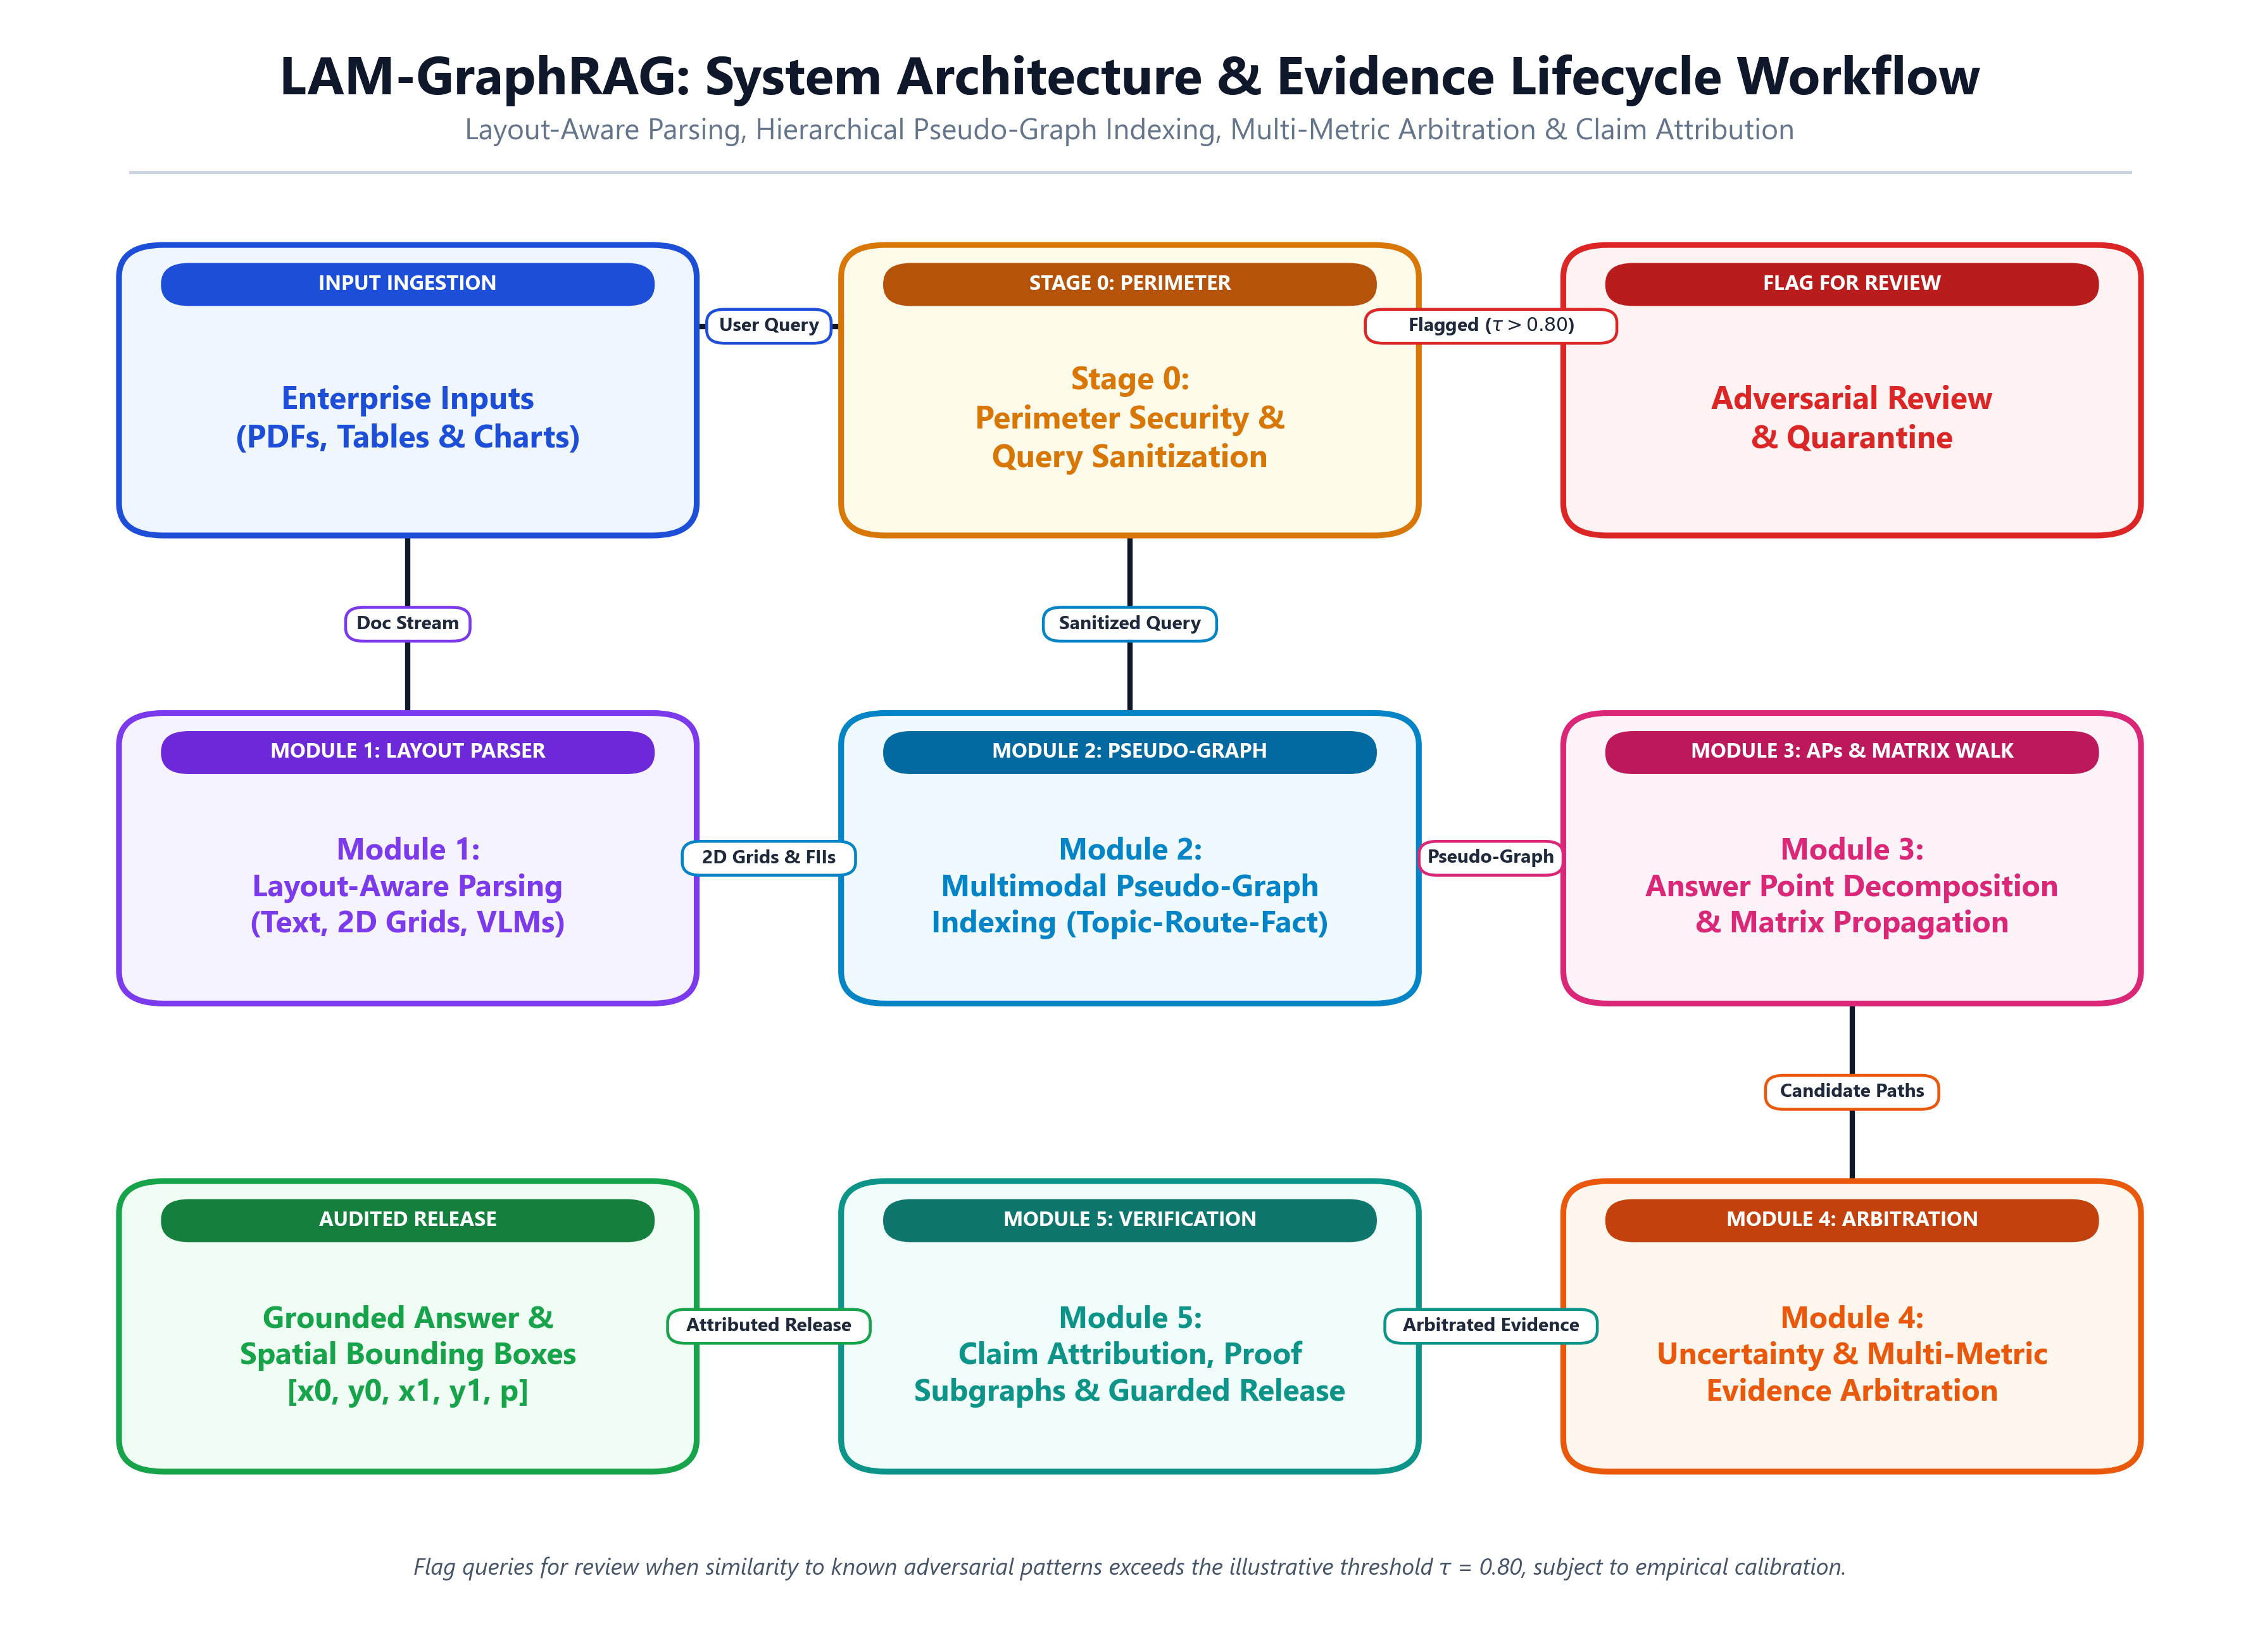
\includegraphics[width=0.98\textwidth]{rag_pipeline_flowchart.png}
\caption{Architectural Blueprint for Layout-Aware Multimodal GraphRAG (LAM-GraphRAG), illustrating the modular execution pipeline (Modules 1--5) preserving coordinate-level evidence provenance from document ingestion to claim verification. Flag queries for review when similarity to known adversarial patterns exceeds the illustrative threshold $\tau = 0.80$, subject to empirical calibration.}
\label{fig:architecture_flowchart}
\end{figure*}

\begin{table*}[t]
\caption{Comparative Analysis of Representative Core Empirical Systems Across the Spatial Evidence Lifecycle.}
\label{tab:empirical}
\centering
\scriptsize
\setlength{\tabcolsep}{2.5pt}
\renewcommand{\arraystretch}{1.12}
\begin{tabularx}{\textwidth}{@{}p{2.1cm}p{1.7cm}p{2.0cm}p{2.1cm}p{1.6cm}c>{\raggedright\arraybackslash}X@{}}
\toprule
\textbf{Study \& Venue} & \textbf{Input Modality} & \textbf{Extraction / Parsing} & \textbf{Graph / Topology} & \textbf{Provenance Unit} & \textbf{Stages} & \textbf{Key Technical Limitation} \\
\midrule
Chen et al. \cite{chen2024tablerag} \newline \emph{NeurIPS '24} & Spreadsheets & Schema \& Cell Filter & Cell-Path Routing & Cell Coordinates & $\mathcal{S}_1, \mathcal{S}_2, \mathcal{S}_4$ & Spreadsheet-only; lacks physical 2D PDF bounding boxes. \\
\addlinespace[1.5pt]
Faysse et al. \cite{faysse2025colpali} \newline \emph{Proc. ICLR '25} & PDF Page Images & PaliGemma Vision & None (Patch Vectors) & Page Level & $\mathcal{S}_2, \mathcal{S}_4$ & High GPU memory footprint; lacks symbolic graph reasoning. \\
\addlinespace[1.5pt]
Huang et al. \cite{huang2022} \newline \emph{ACM MM '22} & Text+Layout+Img & Multimodal Mask & None (Sequence) & 2D Bounding Box & $\mathcal{S}_1$--$\mathcal{S}_3$ & Token-level pretraining; lacks graph multi-hop retrieval. \\
\addlinespace[1.5pt]
Zhao et al. \cite{zhao2024doclayout} \newline \emph{arXiv '24} & Page Bitmaps & YOLOv10 + GL-CRM & None (BBox Grid) & 2D Bounding Box & $\mathcal{S}_1, \mathcal{S}_2$ & Perception only; lacks graph indexing and multi-hop reasoning. \\
\addlinespace[1.5pt]
Wang et al. \cite{wang2024mineru} \newline \emph{arXiv '24} & Multi-Page PDFs & Hybrid Layout+OCR & Markdown Hierarchy & Block / Region & $\mathcal{S}_1, \mathcal{S}_2$ & Strips individual cell bounding boxes in markdown export. \\
\addlinespace[1.5pt]
Niu et al. \cite{niu2026} \newline \emph{IEEE TKDE '26} & Text Corpora & Topic-Route-Fact & In-Memory Pseudo-G & Fact Info Item & $\mathcal{S}_2$--$\mathcal{S}_4$ & Text-focused; lacks visual coordinate anchoring. \\
\addlinespace[1.5pt]
Zhang et al. \cite{zhang2026m2ag} \newline \emph{IEEE TMM '26} & Text + Image & Dynamic Relevance & Reflection Graph & Multimodal Span & $\mathcal{S}_3$--$\mathcal{S}_5$ & Scoped to single-turn VQA; lacks cross-page hierarchy. \\
\addlinespace[1.5pt]
Edge et al. \cite{edge2024} \newline \emph{arXiv '24} & Text Corpora & LLM Extraction & Hierarchical Leiden & Passage Cluster & $\mathcal{S}_3, \mathcal{S}_4$ & Costly LLM triples; discards 2D PDF layout boxes. \\
\addlinespace[1.5pt]
Guo et al. \cite{guo2025lightrag} \newline \emph{Findings EMNLP '25} & Text Corpora & Dual-Level Prompts & Entity-Theme Graph & Graph Node & $\mathcal{S}_3, \mathcal{S}_4$ & Text-only; ignores tabular dependencies and charts. \\
\addlinespace[1.5pt]
Qi et al. \cite{qi2026} \newline \emph{IEEE TKDE '26} & Text + Curated KG & Entity Descriptions & DGHMA Hetero-G & Traversal Path & $\mathcal{S}_3$--$\mathcal{S}_5$ & Assumes curated KG; lacks 2D layout and chart awareness. \\
\addlinespace[1.5pt]
Asai et al. \cite{asai2024selfrag} \newline \emph{Proc. ICLR '24} & Text Corpora & Reflection Tokens & Beam Tree Search & Passage Sub-span & $\mathcal{S}_4, \mathcal{S}_5$ & Requires instruction tuning; lacks coordinate provenance. \\
\bottomrule
\end{tabularx}
\end{table*}

%========================================================================================
% SECTION V: CROSS-PAGE RETRIEVAL & GRAPH REASONING
%========================================================================================
\section{Cross-Page Retrieval and Graph Reasoning (RQ2, RQ3)}

\subsection{Multi-Hop Traversal via Discounted Matrix Propagation}
Iterative Chain-of-Thought prompting \cite{trivedi2023} suffers from error accumulation and prompt runaway. While reflection-based architectures (Self-RAG \cite{asai2024selfrag}, CRAG \cite{yan2024crag}, Adaptive-RAG \cite{jeong2024adaptiverag}) and hybrid knowledge graphs (KAG \cite{liang2024kag}, G-Retriever \cite{he2024gretriever}) regulate text retrieval, they operate largely on ungrounded text strings. In LAM-GraphRAG, we formulate a dedicated \textbf{Answer Point (AP) decomposition component} as an architectural formulation:
\begin{equation}
Q \xrightarrow{\text{Decompose}} \{AP_1, AP_2, \dots, AP_m\}
\label{eq:ap_decomp}
\end{equation}
where each $AP_j$ represents an atomic visual, tabular, or textual sub-intent requiring verification against physical bounding boxes. In parallel, inspired by PG-RAG's hierarchical indexing \cite{niu2026}, documents are indexed as in-memory pseudo-graphs:
\begin{equation}
\mathcal{T}_{\text{doc}} = (\mathcal{V}_{\text{Topic}} \cup \mathcal{V}_{\text{Route}} \cup \mathcal{V}_{\text{Fact}}, \mathcal{E}_{\text{hier}})
\label{eq:pg_rag_tree}
\end{equation}
incorporating associative memory (HippoRAG \cite{gutierrez2024hipporag}), graph convolution \cite{kipf2017}, attention networks \cite{velickovic2018}, and question-answering graphs \cite{yasunaga2021, shen2026rar}. To explore multi-hop reasoning chains deterministically, let $\mathbf{A} \in \mathbb{R}^{|\mathcal{V}| \times |\mathcal{V}|}$ denote the row-stochastic adjacency matrix where $A_{ij} = P(v_j \mid v_i)$ and $\sum_j A_{ij} = 1$. Let $\mathbf{r}_k \in \mathbb{R}^{|\mathcal{V}| \times 1}$ represent a column probability vector over graph nodes at step $k$. Probability mass propagates via the transpose matrix $\mathbf{A}^\top$:
\begin{equation}
\mathbf{r}_0 = \mathbf{E}_{\text{init}}, \quad \mathbf{r}_k = \mathbf{A}^\top \mathbf{r}_{k-1}, \quad \mathbf{R}^{(K)} = \sum_{k=1}^K \delta^k \mathbf{r}_k
\label{eq:matrix_walk}
\end{equation}
where $\delta \in (0, 1)$ is a propagation discount factor and $K$ is a finite exploration horizon (e.g., $K \le 3$). Because $\mathbf{A}$ is sparse ($|\mathcal{E}| \ll |\mathcal{V}|^2$), each sparse matrix-vector multiplication computes in $O(|\mathcal{E}|)$ operations, bounding total exploration complexity strictly to $O(K \cdot |\mathcal{E}|)$. While exact matrix propagation completely avoids Monte Carlo sampling variance, it operates conditioned on estimated edge weights and does not eliminate epistemic uncertainty in the underlying transition probabilities $A_{ij}$.

\subsection{Uncertainty-Aware Evidence Arbitration}
When aggregating multi-hop evidence across visual layouts and text passages, retrieved information often exhibits epistemic uncertainty and conflicting claims \cite{gawlikowski2023}. To mitigate ungrounded propagation, candidate paths $\pi_i$ are ranked using affine-rescaled cosine similarity $\hat{s}(\pi_i, Q) = \frac{1 + \cos(\mathbf{e}_{\pi_i}, \mathbf{e}_Q)}{2} \in [0,1]$ penalized by calibrated epistemic uncertainty $\tilde{\sigma}_{\pi_i} \ge 0$:
\begin{equation}
\text{Score}(\pi_i) = \hat{s}(\pi_i, Q) \cdot \exp(-\lambda \tilde{\sigma}_{\pi_i})
\label{eq:upr}
\end{equation}
where $\lambda \ge 0$ is a risk-aversion hyperparameter. Multi-metric arbitration balances generation and retrieval confidence:
\begin{equation}
\mathcal{A}(y) = \alpha C_m + \beta C_r + \gamma S_c
\label{eq:arbitration}
\end{equation}
where $C_m \in [0,1]$ denotes model generation confidence, $C_r \in [0,1]$ represents cross-source retrieval consistency, and $S_c \in [0,1]$ quantifies spatial-layout coherence, with illustrative conceptual weights $\alpha=0.35, \beta=0.40, \gamma=0.25$ ($\alpha+\beta+\gamma=1$). Crucially, $C_m, C_r,$ and $S_c$ are min-max normalized to the common unit interval $[0,1]$ prior to weighted fusion. Inspired by DUAL-Know's attention principles \cite{qi2026}, our proposed architecture incorporates uncertainty-aware path ranking (Eq.~\ref{eq:upr}) and multi-metric arbitration fusion (Eq.~\ref{eq:arbitration}) into \textbf{Module~4 (Uncertainty \& Multi-Metric Evidence Arbitration)}, resolving epistemic layout conflicts prior to generation.

\subsection{Agentic Safeguards and Security}
Inspired by existing LLM runtime guardrails \cite{tripathi2026, yang2025adaptiveguard}, we bound multi-hop traversal using an execution budget and maximum iteration limit $T_{\max}$ as a circuit-breaker. In parallel, Hu et al.~\cite{hu2025membership} propose a VAE-based query preprocessing mechanism to mitigate membership-inference attacks by moving query representations toward the non-member region of the feature space. TrumorGPT \cite{hang2025trumor} constructs veracity subgraphs to mitigate misinformation. Securing multi-hop reasoning against poisoned or backdoor graph spans \cite{zheng2026trigger} requires explicit confidence calibration and evidence arbitration rather than heuristic stopping rules alone \cite{qi2026}.

%========================================================================================
% SECTION VI: BENCHMARK & EVALUATION ANALYSIS
%========================================================================================
\section{Benchmark and Evaluation Analysis (RQ4)}

\subsection{Decoupling Spatial Localization from Semantic Retrieval}
Standard retrieval evaluations prioritize top-$k$ text recall, masking spatial localization failures. We establish a four-dimensional evaluation taxonomy: (1)~\emph{Text Retrieval (Txt-R)}: measuring passage retrieval (Recall@K, MRR); (2)~\emph{Page-Level Grounding (Doc-G)}: measuring page isolation in multi-page corpora (Page Recall@K); (3)~\emph{Coordinate Localization (Coord-L)}: measuring exact 2D bounding boxes or table cell coordinates ($[x_1, y_1, x_2, y_2]$, CIR, IoU); and (4)~\emph{Claim Attribution (Clm-A)}: measuring factual citation support (ALCE \cite{gao2023alce}, FActScore \cite{min2023factscore}).

\begin{table}[htbp]
\caption{Audit of Nine Representative Benchmarks Relevant to Document Retrieval, Grounding, Reasoning, and Attribution.}
\centering
\scriptsize
\setlength{\tabcolsep}{1.2pt}
\begin{tabularx}{\columnwidth}{@{}p{1.9cm}p{1.3cm}>{\raggedright\arraybackslash}Xcccc@{}}
\toprule
\textbf{Benchmark} & \textbf{Modality} & \textbf{Primary Target} & \textbf{T-R} & \textbf{D-G} & \textbf{C-L} & \textbf{C-A} \\
\midrule
HotpotQA \cite{yang2018hotpotqa} & Pure Text & 2-Hop Fact Chains & $\bullet$ & $\times$ & $\times$ & $\circ$ \\
ChartQA \cite{masry2022} & Chart Images & Visual / Numerical QA$^\ddagger$ & $\times$ & $\times$ & $\times$ & $\times$ \\
ALCE \cite{gao2023alce} & Text Docs & Citation Support & $\bullet$ & $\times$ & $\times$ & $\bullet$ \\
TableRAG \cite{chen2024tablerag} & Spreadsheet & Million-Token Tables$^\dagger$ & $\bullet$ & $\times$ & $\times$ & $\times$ \\
ViDoRe \cite{faysse2025colpali} & Visual Page & Visual Page Retrieval & $\times$ & $\bullet$ & $\times$ & $\times$ \\
M3DocVQA \cite{m3docvqa2025} & Multi-PDF & Multi-Page DocVQA$^*$ & $\circ$ & $\circ$ & $\times$ & $\times$ \\
MMDocRAG \cite{dong2025mmdocrag} & PDF Pages & End-to-End MM-RAG & $\circ$ & $\bullet$ & $\times$ & $\times$ \\
PubTabNet \cite{zhong2020pubtabnet} & Tables & Table Recognition & $\times$ & $\times$ & $\circ^\mathsection$ & $\times$ \\
FActScore \cite{min2023factscore} & Text Docs & Atomic Fact Precision$^*$ & $\times$ & $\times$ & $\times$ & $\circ$ \\
\bottomrule
\end{tabularx}
\vspace{1.5pt}
\begin{minipage}{\columnwidth}
{\scriptsize\raggedright \textbf{Dimensions:} \textbf{T-R} = Text Retrieval; \textbf{D-G} = Document Grounding; \textbf{C-L} = Coordinate Localization; \textbf{C-A} = Claim Attribution. $\bullet$ = Evaluated; $\circ$ = Partial; $\times$ = None. $^\dagger$TableRAG uses logical cell indexing over worksheets rather than PDF bboxes (C-L). $^\ddagger$ChartQA benchmarks chart visual QA without multi-page document provenance. $^*$M3DocVQA annotates page indices; FActScore evaluates claim precision without spatial bounding boxes. $^\mathsection$PubTabNet provides bounding-box annotations in its corpus, but standard benchmark evaluation relies on Tree-Edit-Distance-based Similarity (TEDS) evaluating HTML table structure rather than coordinate localization error.\par}
\end{minipage}
\label{tab:benchmarks}
\end{table}

Table~\ref{tab:benchmarks} presents nine representative benchmarks selected and evaluated against our four proposed evaluation dimensions across document retrieval, visual grounding, coordinate localization, and claim attribution (serving as an analytical cross-section rather than an exhaustive catalog of all extant NLP benchmarks). Crucially, as confirmed in our formal benchmark audit matrix, none of the nine audited benchmarks jointly evaluates physical coordinate localization (Coord-L) and claim attribution (Clm-A), demonstrating an empirically verified void in current multimodal document RAG evaluation.

\subsection{Cross-System Empirical Synthesis}
Table~\ref{tab:empirical} categorizes 11 representative landmark systems across the evidence lifecycle. While visual parsers (LayoutLMv3 \cite{huang2022}, DocLayout-YOLO \cite{zhao2024doclayout}) achieve robust spatial segmentation ($\mathcal{S}_1, \mathcal{S}_2$), they lack relational graph indexing ($\mathcal{S}_3$) and cross-page reasoning ($\mathcal{S}_4$). Conversely, advanced GraphRAG architectures (GraphRAG \cite{edge2024}, LightRAG \cite{guo2025lightrag}, DUAL-Know \cite{qi2026}) provide powerful topological traversal but operate almost exclusively on linearized text passages, discarding 2D bounding boxes. Systems addressing tabular data (TableRAG \cite{chen2024tablerag}) excel at programmatic cell routing but ignore scanned PDF layouts. This systematic dichotomy underscores the necessity of unifying spatial coordinate preservation with topological graph retrieval.

%========================================================================================
% SECTION VII: CONCEPTUAL SYNTHESIS & OPEN CHALLENGES
%========================================================================================
\section{Conceptual Synthesis and Open Challenges (RQ5)}

\subsection{The LAM-GraphRAG Architectural Framework}
To unify spatial layout awareness with graph-structured retrieval, we synthesize the \textbf{Layout-Aware Multimodal GraphRAG (LAM-GraphRAG)} architectural blueprint (Fig.~\ref{fig:architecture_flowchart}):
\begin{itemize}
    \item \textbf{Stage 0 (Perimeter Security):} Ingestion validation, query sanitation \cite{hu2025membership}, and structural anomaly detection for poisoned graphs \cite{zheng2026trigger}.
    \item \textbf{Module 1 (Layout-Aware Parsing):} Combines fast extractors with vision-language parsers (DocLayout-YOLO \cite{zhao2024doclayout}, LayoutLMv3 \cite{huang2022}), anchoring every block, cell, and mark to immutable $[x_0, y_0, x_1, y_1, p]$ page bounding boxes.
    \item \textbf{Module 2 (PG-RAG Multimodal Extension):} Extends PG-RAG's hierarchy \cite{niu2026} to multimodal documents, constructing in-memory Topic, Route, and Fact nodes tagged with spatial bounding boxes.
    \item \textbf{Module 3 (Sub-Intent Decomposition \& Matrix Propagation):} Decomposes queries into explicit Answer Points (APs), our proposed spatial verification targets inspired by sub-intent query parsing \cite{wang2025, zhang2026m2ag}, and executes discounted transition probability walks (Eq.~\ref{eq:matrix_walk}) to discover cross-page bridge entities.
    \item \textbf{Module 4 (Uncertainty \& Multi-Metric Evidence Arbitration):} Executes variance-penalized path ranking (Eq.~\ref{eq:upr}) and multi-metric arbitration fusion (Eq.~\ref{eq:arbitration}) inspired by DUAL-Know \cite{qi2026} to arbitrate conflicting cross-page evidence before generation.
    \item \textbf{Module 5 (Claim Attribution, Proof Subgraphs \& Guarded Release):} Generates final answers where each assertion is bound to active bounding boxes and proof subgraphs, enforcing provenance auditability and guarded release.
\end{itemize}

\subsection{Open Research Challenges}
\begin{enumerate}
    \item \textbf{Continuous Coordinate Embeddings:} Multi-vector models (ColPali \cite{faysse2025colpali}) index patch tokens without continuous coordinate conditioning. Joint layout embeddings retaining sub-patch coordinates without memory explosion remain an open priority.
    \item \textbf{Unified Region-IoU and Claim Attribution Benchmarks:} Existing benchmarks separate visual retrieval from text citation. A unified benchmark jointly penalizing spatial bounding-box error ($\text{IoU} < 0.5$) and claim non-entailment is urgently needed.
    \item \textbf{Scalable Dynamic In-Memory Graphs:} While in-memory pseudo-graphs \cite{niu2026} avoid graph database latency, scaling to million-token document corpora requires dynamic subgraph pruning and hierarchical paging.
\end{enumerate}

%========================================================================================
% SECTION VIII: CONCLUSION & ACKNOWLEDGMENT
%========================================================================================
\section{Conclusion}
To our knowledge, this review provides one of the first structured analyses of spatial provenance, cross-page retrieval, and claim attribution in multimodal document RAG. Following PRISMA 2020 principles, we synthesized 50 research sources (45 database archival studies and 5 supplementary citation-snowballing sources, stratified into 23 core empirical systems and 27 supporting literature sources) from 540 initial records with substantial inter-reviewer reliability ($94.55\%$ and $95.35\%$ agreement, $\kappa = 0.8109$ and $\kappa = 0.9044$). We formalized the five-stage Evidence Lifecycle Framework, defined operational tabular metrics ($\text{CIR}_{\text{logical}}$, $\text{CIR}_{\text{data}}$, H-RCR, C-RCR), formulated bounded multi-hop propagation via discounted transition probability matrices, and confirmed that none of nine audited benchmarks jointly evaluates physical coordinate localization and claim attribution. Finally, we synthesized design principles into Layout-Aware Multimodal GraphRAG (LAM-GraphRAG), establishing an auditable, provenance-grounded roadmap for multimodal document intelligence.

\section*{Acknowledgment}
\begin{samepage}
The authors express their sincere gratitude to the Department of Artificial Intelligence \& Data Science at Vidya Pratishthan's Kamalnayan Bajaj Institute of Engineering and Technology (VPKBIET), Baramati, affiliated with Savitribai Phule Pune University (SPPU), Pune, India. We thank Mrs.~Hema Jadhav for project guidance and research supervision, and Dr.~C.~S.~Kulkarni, Head of Department, for institutional support and infrastructural resources.

\noindent In accordance with IEEE Author Center policy on Artificial Intelligence (AI)-Generated Content, the authors disclose that the Google Antigravity agentic development platform (powered by the Gemini 2.5 Pro language model) was used to assist in grammatical polishing, LaTeX structural formatting, and exploratory search query keyword expansion for Sections~I--III. All literature screening decisions, data extraction parameters, quality appraisals, PRISMA 2020 statistical evaluations, mathematical derivations (Equations 1--8), architectural synthesis, and analytical conclusions were conceived, conducted, and verified independently by the human co-authors, who take full intellectual responsibility for the contents of this manuscript.
\end{samepage}

%========================================================================================
% INLINED CANONICAL BIBLIOGRAPHY (50 Verified Entries - Balanced for Final Page 8)
%========================================================================================
\IEEEtriggeratref{26}
\begingroup
\scriptsize
\setlength{\parskip}{0pt}
\def\IEEEbibitemsep{0.35pt plus 0.15pt minus 0.10pt}
\begin{thebibliography}{50}

\bibitem{qi2026} H. Qi, J. Li, Y. Ge, H. Wu, Y. Cai, S. Che, T. Sheng, Q. Zhao, and C. Chen, ``DUAL-Know: A Description-Augmented and Uncertainty-Aware GraphRAG Framework for Anesthesiology Question Answering,'' \emph{IEEE TKDE, vol. 38, no. 8, pp. 5015--5031, Aug. 2026}, doi: \url{https://doi.org/10.1109/TKDE.2026.3700611}.

\bibitem{niu2026} S. Niu, M. Wang, X. Liang, Z. Li, S. Zhang, S. Song, H. Wang, J. Yang, F. Xiong, and C. Xi, ``Empowering Large Language Models to Set Up Knowledge Retrieval Indexing via Self-Learning,'' \emph{IEEE TKDE, vol. 38, no. 3, pp. 1710--1724, Mar. 2026}, doi: \url{https://doi.org/10.1109/TKDE.2025.3649907}.

\bibitem{zhang2026m2ag} Tao Zhang, Ziqi Zhang, Zongyang Ma, Yuxin Chen, Zhongang Qi, et al., ``mR²AG: Multimodal Retrieval-Reflection-Augmented Generation for Knowledge-Based VQA,'' \emph{IEEE TMM, vol. 28, pp. 2450--2463, 2026}, doi: \url{https://doi.org/10.1109/TMM.2026.3723597}.

\bibitem{shen2026rar} Xiangqing Shen, Fanfan Wang, Zinong Yang, Bing Wang, Wenli Du, Chengqing Zong, and Rui Xia, ``Reason-Align-Respond: Aligning LLM Reasoning With Knowledge Graphs for KGQA,'' \emph{IEEE TPAMI, vol. 48, no. 7, pp. 7340--7353, Jul. 2026}, doi: \url{https://doi.org/10.1109/TPAMI.2026.3665645}.

\bibitem{hang2025trumor} Ching Nam Hang, Pei-Duo Yu, and Chee-Wei Tan, ``TrumorGPT: Graph-Based Retrieval-Augmented Large Language Model for Fact-Checking and Misinformation Mitigation,'' \emph{IEEE TAI, vol. 6, no. 4, pp. 1820--1834, 2025}, doi: \url{https://doi.org/10.1109/TAI.2025.3567369}.

\bibitem{zheng2026trigger} Zhirun Zheng, Young-June Choi, Cheng Huang, Hangcheng Cao, Shujuan Tian, and Tingrui Pei, ``Trigger as Entity: Backdoor Attacks to Graph-Based Retrieval-Augmented Generation of Large Language Models,'' \emph{IEEE TIFS, vol. 21, pp. 5583--5596, 2026}, doi: \url{https://doi.org/10.1109/TIFS.2026.3699202}.

\bibitem{lewis2020} Patrick Lewis, Ethan Perez, Aleksandra Piktus, Fabio Petroni, et al., ``Retrieval-Augmented Generation for Knowledge-Intensive NLP Tasks,'' \emph{NeurIPS, vol. 33, pp. 9459--9474, 2020}, doi: \url{https://doi.org/10.5555/3495724.3496517}.

\bibitem{edge2024} Darren Edge, Ha Trinh, Newman Cheng, Joshua Bradley, Alex Chao, et al., ``From Local to Global: A Graph RAG Approach to Query-Focused Summarization,'' \emph{arXiv preprint, 2024}, \url{https://arxiv.org/abs/2404.16130}.

\bibitem{guo2025lightrag} Zirui Guo, Lianghao Xia, Yanhua Yu, Tu Ao, and Chao Huang, ``LightRAG: Simple and Fast Retrieval-Augmented Generation,'' \emph{Findings of EMNLP, pp. 10746--10761, 2025}, doi: \url{https://doi.org/10.18653/v1/2025.findings-emnlp.568}.

\bibitem{huang2022} Yupan Huang, Tengchao Lv, Lei Cui, Yutao Lu, and Furu Wei, ``LayoutLMv3: Pre-training for Document AI with Unified Text and Image Masking,'' \emph{Proc. ACM MM, pp. 4083--4091, 2022}, doi: \url{https://doi.org/10.1145/3503161.3548112}.

\bibitem{tripathi2026} P. Tripathi, P. Arora, K. K. Paroha, D. Kumar, Manisha, and P. Katiyar, ``Guardrail-Based Approaches for Enhancing Safety, Security, and Privacy in Large Language Models,'' \emph{IEEE IC3ECSBHI, pp. 1619--1624, 2026}, doi: \url{https://doi.org/10.1109/IC3ECSBHI67834.2026.11469093}.

\bibitem{yang2025adaptiveguard} Rui Yang, Michael Fu, Chakkrit Tantithamthavorn, Chetan Arora, Gunel Gulmammadova, and Joey Chua, ``AdaptiveGuard: Towards Adaptive Runtime Safety for LLM-Powered Software,'' \emph{Proc. 40th IEEE/ACM ASE, pp. 3381--3391, 2025}, doi: \url{https://doi.org/10.1109/ASE63991.2025.00279}.

\bibitem{hu2025membership} L. Hu, H. Yan, Y. Peng, H. Hu, S. Wang, and J. Li, ``VAE-Based Membership Cleanser Against Membership Inference Attacks,'' \emph{IEEE TDSC, vol. 22, no. 2, pp. 1253--1264, Mar.-Apr. 2025}, doi: \url{https://doi.org/10.1109/TDSC.2024.3429203}.

\bibitem{wang2025} Yuchen Wang, Haolong Wang, Kai Wang, and Xinyu Du, ``Decomposed Modular RAG: Task-Aware Multi-Step Retrieval and Reasoning for Small-Scale Language Models,'' \emph{Proc. 2025 8th IEEE CISAT, pp. 128--133, 2025}, doi: \url{https://doi.org/10.1109/CISAT66811.2025.11181923}.

\bibitem{gao2026} Sensen Gao, Shanshan Zhao, Xu Jiang, Lunhao Duan, Yong Xien Chng, et al., ``Scaling Beyond Context: A Survey of Multimodal Retrieval-Augmented Generation for Document Understanding,'' \emph{Proc. 64th ACL, pp. 4458--4489, 2026}, doi: \url{https://doi.org/10.18653/v1/2026.acl-long.204}.

\bibitem{gawlikowski2023} J. Gawlikowski, C. R. N. Tassi, M. Ali, J. Lee, M. Humt, J. Feng, A. Kruspe, R. Triebel, et al., ``A Survey of Uncertainty in Deep Neural Networks,'' \emph{Information Fusion, vol. 100, art. no. 101978, 2023}, doi: \url{https://doi.org/10.1016/j.inffus.2023.101978}.

\bibitem{ji2023} Ziwei Ji, Nayeon Lee, Rita Frieske, Tiezheng Yu, Dan Su, Yan Xu, et al., ``Survey of Hallucination in Natural Language Generation,'' \emph{ACM Comput. Surv. (CSUR), vol. 55, no. 12, pp. 1--38, 2023}, doi: \url{https://doi.org/10.1145/3571730}.

\bibitem{yang2018hotpotqa} Zhilin Yang, Peng Qi, Saizheng Zhang, Yoshua Bengio, William W. Cohen, Ruslan Salakhutdinov, and Christopher D. Manning, ``HotpotQA: A Dataset for Diverse, Explainable Multi-Hop Question Answering,'' \emph{Proc. EMNLP, pp. 2369--2380, 2018}, doi: \url{https://aclanthology.org/D18-1259}.

\bibitem{yasunaga2021} Michihiro Yasunaga, Hongyu Ren, Antoine Bosselut, Percy Liang, and Jure Leskovec, ``QA-GNN: Reasoning with Language Models and Knowledge Graphs for Question Answering,'' \emph{Findings of ACL: NAACL, pp. 273--288, 2021}, doi: \url{https://aclanthology.org/2021.findings-naacl.24}.

\bibitem{chen2024tablerag} Si-An Chen, Lesly Miculicich, Julian Martin Eisenschlos, Zifeng Wang, Zilong Wang, Yanfei Chen, Yasuhisa Fujii, Hsuan-Tien Lin, Chen-Yu Lee, and Tomas Pfister, ``TableRAG: Million-Token Table Understanding with Language Models,'' \emph{NeurIPS, vol. 37, pp. 74899--74921, 2024}, doi: \url{https://doi.org/10.52202/079017-2382}.

\bibitem{devlin2019} Jacob Devlin, Ming-Wei Chang, Kenton Lee, and Kristina Toutanova, ``BERT: Pre-training of Deep Bidirectional Transformers for Language Understanding,'' \emph{Proc. NAACL-HLT, pp. 4171--4186, 2019}, doi: \url{https://aclanthology.org/N19-1423}.

\bibitem{brown2020} Tom B. Brown, Benjamin Mann, Nick Ryder, Melanie Subbiah, et al., ``Language Models are Few-Shot Learners,'' \emph{NeurIPS, vol. 33, pp. 1877--1901, 2020}, doi: \url{https://doi.org/10.5555/3495724.3495883}.

\bibitem{radford2021} Alec Radford, Jong Wook Kim, Chris Hallacy, Aditya Ramesh, et al., ``Learning Transferable Visual Models From Natural Language Supervision,'' \emph{Proc. 38th ICML, pp. 8748--8763, 2021}, doi: \url{https://doi.org/10.5555/3495724.3496460}.

\bibitem{liu2023llava} Haotian Liu, Chunyuan Li, Qingyang Wu, and Yong Jae Lee, ``Visual Instruction Tuning,'' \emph{NeurIPS, vol. 36, pp. 34979--35016, 2023}, doi: \url{https://doi.org/10.52202/069902-1118}.

\bibitem{liu2024lost} Nelson F. Liu, Kevin Lin, John Hewitt, Ashwin Paranjape, Michele Bevilacqua, Fabio Petroni, and Percy Liang, ``Lost in the Middle: How Language Models Use Long Contexts,'' \emph{Trans. Assoc. Comput. Linguistics (TACL), vol. 12, pp. 157--173, 2024}, doi: \url{https://doi.org/10.1162/tacl\_a\_00638}.

\bibitem{kipf2017} Thomas N. Kipf and Max Welling, ``Semi-Supervised Classification with Graph Convolutional Networks,'' \emph{Proc. 5th ICLR, pp. 1--14, 2017}, \url{https://arxiv.org/abs/1609.02907}.

\bibitem{velickovic2018} Petar Veličković, Guillem Cucurull, Arantxa Casanova, Adriana Romero, Pietro Liò, and Yoshua Bengio, ``Graph Attention Networks,'' \emph{Proc. 6th ICLR, pp. 1--12, 2018}, \url{https://arxiv.org/abs/1710.10903}.

\bibitem{zhong2020pubtabnet} Xu Zhong, Elaheh ShafieiBavani, and Antonio Jimeno Yepes, ``Image-Based Table Recognition: Data, Model, and Evaluation,'' \emph{Proc. 16th ECCV, pp. 564--580, 2020}, doi: \url{https://doi.org/10.1007/978-3-030-58589-1\_34}.

\bibitem{trivedi2023} Harsh Trivedi, Niranjan Balasubramanian, Tushar Khot, and Ashish Sabharwal, ``Interleaving Retrieval with Chain-of-Thought Reasoning for Knowledge-Intensive Multi-Step Questions,'' \emph{Proc. 61st ACL, pp. 10001--10020, 2023}, doi: \url{https://aclanthology.org/2023.acl-long.557}.

\bibitem{guu2020} Kelvin Guu, Kenton Lee, Zora Tung, Panupong Pasupat, and Ming-Wei Chang, ``REALM: Retrieval-Augmented Language Model Pre-Training,'' \emph{Proc. 37th ICML, pp. 3929--3938, 2020}, doi: \url{https://doi.org/10.5555/3524938.3525303}.

\bibitem{gutierrez2024hipporag} Bernal Jiménez Gutiérrez, Yiheng Shu, Yu Gu, Michihiro Yasunaga, and Yu Su, ``HippoRAG: Neurobiologically Inspired Long-Term Memory for Large Language Models,'' \emph{NeurIPS, vol. 37, pp. 59532--59569, 2024}, doi: \url{https://doi.org/10.52202/079017-1902}.

\bibitem{faysse2025colpali} Manuel Faysse, Hugues Sibille, Tony Wu, Bilel Omrani, Gautier Viaud, Céline Hudelot, and Pierre Colombo, ``ColPali: Efficient Document Retrieval with Vision Language Models,'' \emph{Proc. 13th ICLR, pp. 1--21, 2025}, \url{https://arxiv.org/abs/2407.01449}.

\bibitem{zhao2024doclayout} Zhiyuan Zhao, Hengrui Kang, Bin Wang, and Conghui He, ``DocLayout-YOLO: Enhancing Document Layout Analysis through Diverse Synthetic Data and Global-to-Local Adaptive Perception,'' \emph{arXiv preprint, 2024}, \url{https://arxiv.org/abs/2410.12628}.

\bibitem{masry2022} Ahmed Masry, Do Xuan Long, Jia Qing Tan, Shafiq Joty, and Enamul Hoque, ``ChartQA: A Benchmark for Question Answering about Charts with Visual and Logical Reasoning,'' \emph{Findings of ACL, pp. 2263--2279, 2022}, doi: \url{https://aclanthology.org/2022.findings-acl.177}.

\bibitem{peng2025} Boci Peng, Yun Zhu, Yongchao Liu, Xiaohe Bo, Haizhou Shi, Chuntao Hong, Yan Zhang, and Siliang Tang, ``Graph Retrieval-Augmented Generation: A Survey,'' \emph{ACM Trans. Inf. Syst. (TOIS), vol. 44, no. 2, art. 35, pp. 1--52, 2026}, doi: \url{https://doi.org/10.1145/3777378}.

\bibitem{zhang2025} Xiantao Zhang, ``Roles of MLLMs in Visually Rich Document Retrieval for RAG: A Survey,'' \emph{Proc. 1st IJCNLP-AACL, pp. 19--36, 2025}, doi: \url{https://aclanthology.org/2025.ijcnlp-long.2}.

\bibitem{li2025} Minghan Li, Yishuai Zhang, Tianrui Lv, Siqi Zhao, Miyang Luo, Ercong Nie, and Guodong Zhou, ``A Survey of Long-Document Retrieval in the PLM and LLM Era,'' \emph{ACM Trans. Inf. Syst. (TOIS), vol. 44, no. 8, pp. 1--48, 2026}, doi: \url{https://doi.org/10.1145/3849382}.

\bibitem{ni2026trustworthy} Bo Ni, Zheyuan Liu, Yongjia Lei, Leyao Wang, Yuying Zhao, et al., ``Towards Trustworthy Retrieval Augmented Generation for Large Language Models: A Survey,'' \emph{ACM Comput. Surv. (CSUR), vol. 58, no. 15, pp. 1--36, 2026}, doi: \url{https://doi.org/10.1145/3837074}.

\bibitem{page2021prisma} M. J. Page, J. E. McKenzie, P. M. Bossuyt, I. Boutron, T. C. Hoffmann, et al., ``The PRISMA 2020 Statement: An Updated Guideline for Reporting Systematic Reviews,'' \emph{BMJ, vol. 372, art. no. n71, 2021}, doi: \url{https://doi.org/10.1136/bmj.n71}.

\bibitem{m3docvqa2025} Jaemin Cho, Debanjan Mahata, Ozan Irsoy, Yujie He, and Mohit Bansal, ``M3DocVQA: Multi-modal Multi-page Multi-document Understanding,'' \emph{Proc. IEEE/CVF ICCV Workshops, pp. 6237--6247, 2025}, doi: \url{https://doi.org/10.1109/ICCVW69036.2025.00649}.

\bibitem{dong2025mmdocrag} Kuicai Dong, Yujing Chang, Shijie Huang, Yasheng Wang, Ruiming Tang, and Yong Liu, ``Benchmarking Retrieval-Augmented Multimodal Generation for Document Question Answering,'' \emph{NeurIPS, vol. 38, pp. 20855--20912, 2025}, doi: \url{https://doi.org/10.52202/085713-0619}.

\bibitem{gao2023alce} Tianyu Gao, Howard Yen, Jiatong Yu, and Danqi Chen, ``Enabling Large Language Models to Generate Text with Citations,'' \emph{Proc. EMNLP, pp. 10777--10799, 2023}, doi: \url{https://aclanthology.org/2023.emnlp-main.666}.

\bibitem{asai2024selfrag} Akari Asai, Zeqiu Wu, Yizhong Wang, Avirup Sil, and Hannaneh Hajishirzi, ``Self-RAG: Learning to Retrieve, Generate, and Critique through Self-Reflection,'' \emph{Proc. 12th ICLR, pp. 1--23, 2024}, \url{https://arxiv.org/abs/2310.11511}.

\bibitem{yan2024crag} S.-Q. Yan, J.-C. Gu, Y. Zhu, and Z.-H. Ling, ``Corrective Retrieval Augmented Generation,'' in \emph{Findings of the Association for Computational Linguistics: IJCNLP-AACL 2026}, pp. 2991--3003, doi: \url{https://doi.org/10.18653/2026.findings-aacl.151}.

\bibitem{jeong2024adaptiverag} Soyeong Jeong, Jinheon Baek, Sukmin Cho, Sung Ju Hwang, and Jong C. Park, ``Adaptive-RAG: Determining When and How to Retrieve for Large Language Models,'' \emph{Proc. NAACL, pp. 2941--2956, 2024}, doi: \url{https://aclanthology.org/2024.naacl-long.161}.

\vfill\null\columnbreak
\bibitem{wang2024mineru} Bin Wang, Chao Xu, Xiaomeng Zhao, Linke Ouyang, and Fan Wu, ``MinerU: An Open-Source Solution for Precise Document Content Extraction,'' \emph{arXiv preprint, 2024}, \url{https://arxiv.org/abs/2409.18839}.

\bibitem{blecher2023nougat} Lukas Blecher, Guillem Cucurull Preixens, Thomas Scialom, and Robert Stojnic, ``Nougat: Neural Optical Understanding for Academic Documents,'' in \emph{Proc. 12th Int. Conf. Learn. Representations (ICLR)}, 2024, \url{https://openreview.net/forum?id=v3t5ZBp0Mw}.

\bibitem{he2024gretriever} Xiaoxin He, Yijun Tian, Yifei Sun, Nitesh V. Chawla, Thomas Laurent, Yann LeCun, Xavier Bresson, Bryan Hooi, ``G-Retriever: Retrieval-Augmented Generation for Textual Graph Understanding and Question Answering,'' \emph{Proc. 38th NeurIPS, pp. 132876--132907, 2024}, doi: \url{https://doi.org/10.52202/079017-4224}.

\bibitem{liang2024kag} Lei Liang, Zhongpu Bo, Zhengke Gui, Zhongshu Zhu, Ling Zhong, Peilong Zhao, Mengshu Sun, Zhiqiang Zhang, Jun Zhou, Wenguang Chen, Wen Zhang, and Huajun Chen, ``KAG: Boosting LLMs in Professional Domains via Knowledge Augmented Generation,'' \emph{Companion Proc. ACM Web Conf. (WWW), pp. 334--343, 2025}, doi: \url{https://doi.org/10.1145/3701716.3715240}.

\bibitem{min2023factscore} Sewon Min, Kalpesh Krishna, Xinxi Lyu, Mike Lewis, Wen-tau Yih, Pang Wei Koh, Mohit Iyyer, Luke Zettlemoyer, and Hannaneh Hajishirzi, ``FActScore: Fine-Grained Atomic Evaluation of Factual Precision in Long Form Text Generation,'' \emph{Proc. EMNLP, pp. 12076--12099, 2023}, doi: \url{https://aclanthology.org/2023.emnlp-main.741}.

\end{thebibliography}
\endgroup

\end{document}
